\clearpage
\chapter{Rhythm, Phrase and Form: Advanced}
\label{chap:rhythm-phrase-form}

\subsection*{What you can do after this chapter}
\begin{itemize}
  \item Tell 6/8 from 3/4 by ear and notate a hemiola (three against two) without corrupting the metre.
  \item Split an eight-bar passage into motif--development--phrase--cadence and mark the phrase peak and closing beat.
  \item Label a 16-bar structure as verse/chorus/bridge and explain each section's rhythmic job, not just its name.
  \item In Yeban, make four variations of one motif (sequence, inversion, augmentation, fragmentation) and assemble eight bars.
\end{itemize}

\subsection{6/8 is not ``six beats of four per bar''}

3/4 has three equal beats; 6/8 is a compound metre of two large beats, each containing three eighths. To the ear 3/4 feels like a waltz, 6/8 like a swaying barcarolle. Decide where the ``large beat'' sits before writing:

\begin{center}
\small
\begin{tabular}{clll}
\toprule
Metre & Large beat & Subdivision & Typical use \\
\midrule
3/4 & three quarter-note beats & halves/quarters per beat & waltz, three-beat march \\
6/8 & two large beats (three eighths each) & three eighths per large beat & barcarolle, lyrical chorus, swing \\
12/8 & four large beats (three eighths each) & slow blues, gospel & triple feel per beat \\
\bottomrule
\end{tabular}
\end{center}

A hemiola temporarily hears ``two groups of three'' as ``three groups of two'' (or the reverse). In 6/8, cutting each large beat in half creates a 3/4 illusion; in 3/4, stretching two groups into three each creates a 6/8 illusion. Place a hemiola near a phrase ending to suggest a coming section change.

\begin{figure}[htbp]
\centering
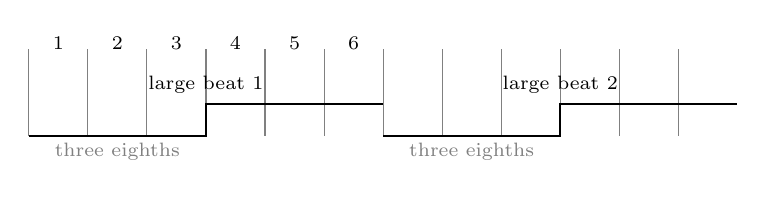
\begin{tikzpicture}[x=0.75cm,y=0.5cm,font=\scriptsize]
  \foreach \b in {0,...,11} { \draw[gray] (\b,0)--(\b,2.2); }
  \foreach \b/\lab in {0/1,1/2,2/3,3/4,4/5,5/6} { \node at (\b+0.5,2.35) {\lab}; }
  \draw[thick] (0,0)--(3,0)--(3,0.8)--(6,0.8);
  \draw[thick] (6,0)--(9,0)--(9,0.8)--(12,0.8);
  \node at (3,1.3) {large beat 1};
  \node at (9,1.3) {large beat 2};
  \node[gray] at (1.5,-0.4) {three eighths};
  \node[gray] at (7.5,-0.4) {three eighths};
\end{tikzpicture}
\caption*{Figure 12-1: The two large beats of 6/8. Each contains three eighths; do not treat the six eighths as six independent beats.}
\end{figure}

\subsection{Groove: accents, syncopation and three-against-two}

Groove is not a pattern name; it is the combination of accent cycle, timbre and duration. Three working rules:

\begin{enumerate}
  \item \textbf{Move the accent}: push a strong-beat accent earlier or later by half a beat to create syncopation; leave a landing note on the next beat, or the line floats away.
  \item \textbf{Three against two}: in 4/4, let one voice run triplets and another run eighths, producing 3:2; both need a stable period, not randomness.
  \item \textbf{Leave space}: after continuous syncopation, leave half a beat empty so the ear can re-align; syncopating every beat makes the section lose direction.
\end{enumerate}

Sketch an ``accent map'' first: mark strong, weak, secondary-strong and weak in each bar, then compare melodic accents with drum accents. If every accent lands on the same beat, the groove is flat; if every beat is syncopated, it scatters.

\subsection{Phrase: motif, peak and cadence}

A phrase is a melodic unit that can breathe on its own, usually two to four bars. Analyse three things:

\begin{itemize}
  \item \textbf{Motif}: the shortest recognisable figure, usually two to five notes;
  \item \textbf{Phrase peak}: the beat of highest tension or densest information, often the top of a sequence;
  \item \textbf{Cadence}: how it closes: half cadence (on V), authentic (V--I), plagal (IV--I), deceptive (V--vi).
\end{itemize}

Four basic ways to develop a motif:

\begin{center}
\small
\begin{tabular}{cll}
\toprule
Device & Operation & Aural effect \\
\midrule
Sequence & move the whole figure up/down & drive, predictability \\
Inversion & reverse interval direction & familiar yet strange \\
Augmentation & stretch durations & emphasis, closing \\
Fragmentation & take only half the motif & acceleration, tension \\
\bottomrule
\end{tabular}
\end{center}

\subsection{Form: the job of a section, not its label}

A common 16-bar structure may be AABA, verse--chorus, or intro--verse--chorus--bridge--outro. The label matters less than each section's rhythmic/harmonic job:

\begin{itemize}
  \item \textbf{Verse}: narrative, lower tension, steadier rhythm, often I--vi--IV--V or a loop;
  \item \textbf{Chorus}: the hook, denser or higher rhythm, harmony often returns to I, strong cadence at the end;
  \item \textbf{Bridge}: contrast, rhythm may slow or speed up, harmony often borrows or modulates;
  \item \textbf{Transition}: use hemiola, syncopation or an ascending sequence to carry the ear into the next section.
\end{itemize}

Eight bars can split as ``2+2+4'': two bars establish the motif, two bars sequence/invert it, four bars deliver the peak and cadence. If all eight bars share one rhythmic pattern, it sounds like a loop; if the metre changes every two bars, it sounds like an exercise.

\subsection{Exercises}
\begin{enumerate}
  \item 6/8 and 3/4 both contain six eighths; why do they sound different?\\
  \emph{Answer:} 6/8 groups them into two large beats of three eighths; 3/4 has three equal quarter beats; the accent cycle differs.
  \item Write a two-bar 4/4 rhythm whose second bar implies 3/4 through hemiola.\\
  \emph{Sample:} bar 1 evenly four beats; bar 2 groups eighths as 3+3+2.
  \item Apply sequence, inversion and augmentation to the four-note motif ``1 2 3 5''.\\
  \emph{Sample:} sequence 2 3 4 6; inversion 1 7 6 4 (axis 1); augmentation 1 1 2 2 3 3 5 5 (double durations).
  \item Analyse an eight-bar passage and mark its peak and cadence type.\\
  \emph{Answer:} the peak is usually the sequence top or highest note; read the last two bars' bass and chords: V--I authentic, V--vi deceptive.
  \item Why leave space after continuous syncopation?\\
  \emph{Answer:} so the listener can re-align to the beat; syncopation with no landing loses direction.
  \item In Yeban, make sequence, inversion, augmentation and fragmentation of ``1 2 3 5'' and assemble eight bars; at least one variation must change metre or add a hemiola.\\
  \emph{Sample:} bars 1--2 original, 3--4 sequence, 5--6 inversion, 7--8 augmentation plus fragmentation; bar 8 closes with a 3+3+2 hemiola.
\end{enumerate}

\subsection{Help topic mapping}
\begin{center}
\footnotesize
\setlength{\tabcolsep}{3pt}
\begin{longtable}{p{0.34\linewidth}p{0.45\linewidth}p{0.15\linewidth}}
\toprule
Section & In-app help anchor & Note \\
\midrule
\endhead
6/8 and hemiola & \texttt{music-theory-compound-meter} & Figure 12-1 \\
Accents and 3:2 & \texttt{music-theory-groove-hemiola} & Rules \\
Phrase and motif & \texttt{music-theory-phrase-motif} & Table 12-1 \\
Section jobs & \texttt{music-theory-section-function} & Structure \\
How to do it in Yeban & \texttt{music-theory-motif-variations} & Operation \\
Exercises & \texttt{music-theory-ch12-practice} & Answers in this chapter \\
\bottomrule
\end{longtable}
\end{center}
